\section{Introdução e Justificativas}\label{Intro}


%=============================================================================
% 							INTRODUÇÃO
%=============================================================================
O debate em torno da distribuição de renda e desigualdade tem retomado o fôlego com a publicação do livro ``\textit{O capital no século XXI}'' de \textcite{piketty_o_2014}. 
Grosso modo, o autor partiu dos dados tributários para verificar a evolução da distribuição de renda e da riqueza, e concluiu que houve um aumento da desigualdade e pior da distribuição de renda nesses países. A razão desta dinâmica, argumenta, decorre da maior remuneração do capital em relação à taxa de crescimento da economia. Esse movimento gerou, no longo prazo, uma maior concentração nos estrados mais altos de renda.
%Não cabe aqui fazer uma leitura crítica desta obra, mas sim pontuar sua relevância no debate recente. Além disso, é importante destacar que os esforços do autor e de sua equipe foram reunidos na divulgação da base de dados referentes a diversos países \cite{alvaredo_wid_nodate}.
Em certa medida, parte da literatura que abordava estes temas passou a utilizar e questionar esses resultados. As publicações que abordam o Brasil não foram exceção\footnote{Uma abordagem semelhante à de \textcite{piketty_o_2014} pode ser encontrada em \textcite{mila_income_2015}. Neste estudo, encontram-se evidências que categorizam o Brasil como um dos países mais desiguais do mundo.}.



Por mais que não seja uma metodologia inédita\footnote{O próprio \textcite{piketty_o_2014} reconhece que não foi pioneiro desta abordagem.}, ela tem lançado luz sobre algumas questões. Os dados referentes ao Imposto sobre a Renda da Pessoa Física (IRPF) permitiram elucidar e explicitar as diferenças nos resultados entre as pesquisas domiciliares em que se verificou uma subestimação da renda dos mais ricos \cites{afonso_irpf_2014}{medeiros_upper_2015}. Com esses novos resultados, põe-se em questão o grau de melhora redistributiva observada no país.

%A ideia de que a dívida pública é um instrumento concentrador de renda foi outra contribuição de \textcite{piketty_o_2014} aplicada ao caso brasileiro. Autores nessa linha, tal como \textcite{dowbor_era_2017}, argumentam que o capitalismo contemporâneo (financeirizado) possui mecanismos que inibem o uso produtivo do capital de tal forma a obstruir o crescimento econômico com geração de empregos. 
%Em linhas gerais, essa corrente argumentativa defende o aprimoramento de instrumentos regulatórios para fazer com que a dinâmica econômica possa retornar para as relações pré-financeirização e, com isso, retomar a autonomia e a soberania  das economias  periféricas \cite{paulani_nao_2017}. 

Além disso, estudos recentes analisando a economia norte-americana reportam a importância da distribuição de renda na determinação da dinâmica econômica. \textcite{grossmann-wirth_role_2018}, por exemplo, explicam a lenta recuperação dos EUA à partir da redução do consumo das famílias no pós Grande Recessão. Neste estudo, os autores concluem que o consumo privado não tem a capacidade de se basear no endividamento tal como antes.

O endividamento das famílias norte-americanas mencionado também pode ser entendido à partir da piora na distribuição de renda. \textcite{barba_rising_2009} argumentam que a estagnação dos salários fez com que as famílias, para manterem determinado padrão relativo de consumo, se endividassem. Com isso, houve um processo de substituição das rendas do trabalho por empréstimos, permitindo que o crescimento econômico se baseasse no consumo privado. Em outras palavras, o aumento do endividamento das famílias é resultado de mudanças persistentes na distribuição e da desigualdade de renda. 


Como contrapartida, verifica-se uma redução significativa da poupança privada. Por conta desta dinâmica, evidencia-se a importância do crédito que, ao permitir um padrão de crescimento pautado no consumo privado, torna possível os trabalhadores gastarem aquilo que não ganham \cite{serrano_trabajadores_2008}. 
Além disso, é importante frisar que este aumento do endividamento das famílias estado-uni\-denses esteve concentrado nos estratos de menor renda. Partindo desta constatação, \textcite{stockhammer_rising_2015} conclui que a Grande Recessão é resultado tanto da desregulamentação financeira quanto dos efeitos macroeconômicos da desigualdade. 

Nesses termos, a experiência norte-americana recente sugere que o endividamento das famílias pode ter resultados macroeconômicos distintos no curto, médio e longo prazo. 
Dessa forma, mostra-se como o aumento do serviço da dívida privada em termos da renda disponível quando acompanhado de uma piora da distribuição de renda pode gerar processos dinamicamente insustentáveis. Sendo assim, fica mais do que evidente a importância de se discutir as relações entre distribuição de renda e crescimento.
Além disso, destaca-se que com o deflagrar da Grande Recessão, boa parte da corrente heterodoxa passou a se preocupar tanto com o consumo das famílias quanto com o endividamento privado \cite{brochier_macroeconomics_2017}.  Esta investigação é, portanto, reflexo deste movimento geral, mas com ênfase no caso brasileiro.

Deste modo, procura-se evidenciar alguns elementos que esclarecem a performance da economia brasileira tendo em vista transformação distributiva observada. Para ilustrar essa dinâmica para o Brasil, o gráfico \ref{path} apresenta a trajetória da participação dos 10\% mais ricos em relação aos 40\% mais pobres acompanhada do comprometimento da Massa Salarial Disponível Ampliada com o serviço da dívida\footnote{Vale destacar os efeitos negativos sobre a distribuição de renda decorrentes da crise financeira internacional internalizada nos anos 2009-10, causando uma mudança brusca no gráfico \ref{path}.}. Deste gráfico, observa-se dois movimentos correlatos: (i) perda da participação relativa dos mais ricos e (ii) crescente endividamento das famílias.

%\begin{figure}[H] % Inicia o ambiente de figuras
%	\begin{center}
%		\caption{Endividamento e participação relativa na renda (2005-2014)}
%		\label{Distri}
%		\subfigure[Endividamento das famílias em relação à Massa Sarial Disponível Ampliada]{ % Começa a incluir a figura fig1.pdf
%			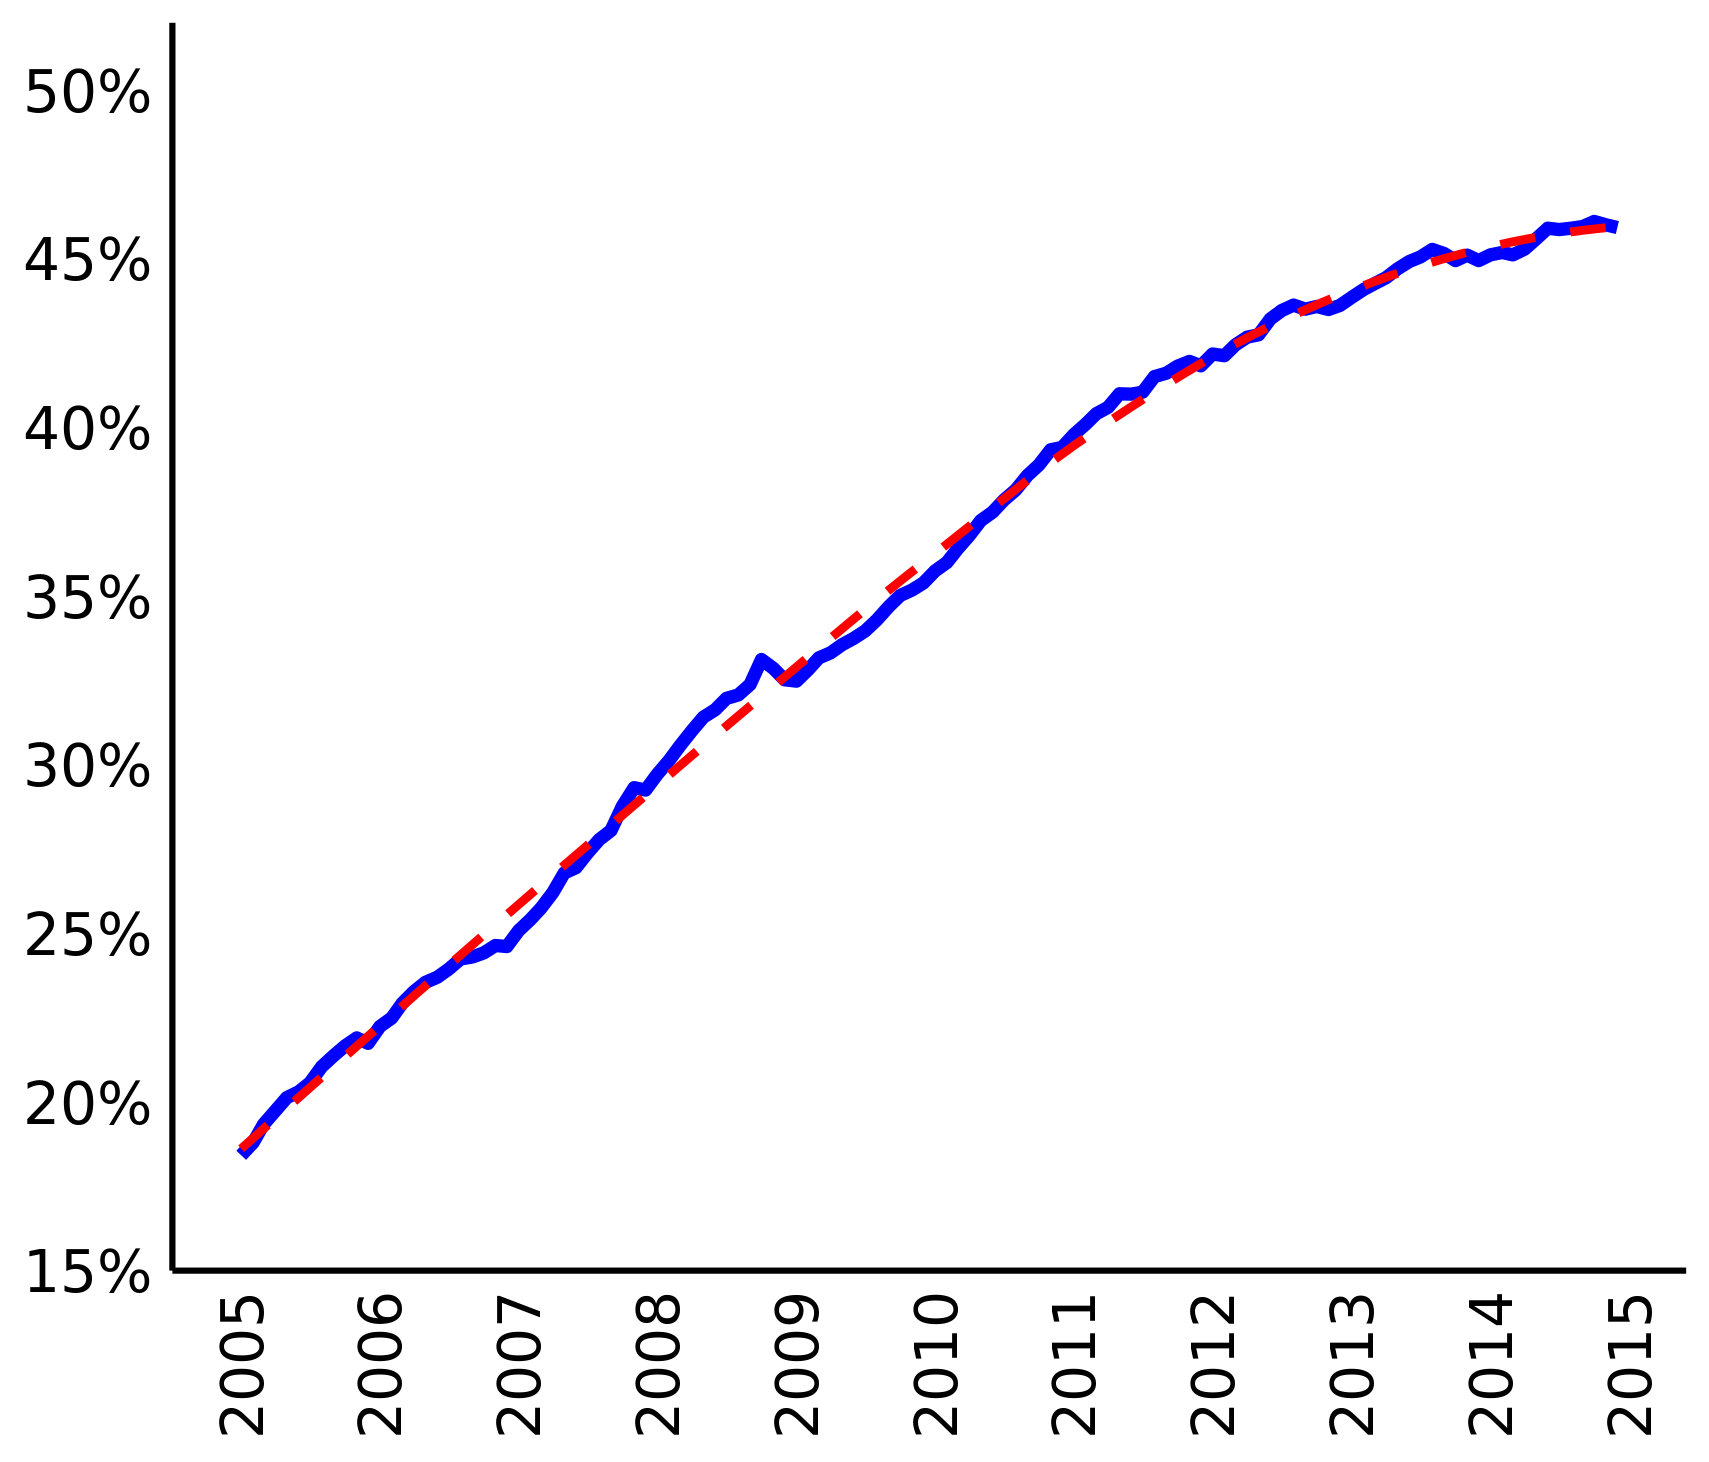
\includegraphics[height=1.8in]{2018-07-23_Plot_Endiv_PIB_FAPESP2.png}\label{Part}
%		} % Termina de incluir a figura fig1.pdf
%		\subfigure[Razão entre a renda dos 10\% mais ricos e dos 40\% mais pobres (2006-2014)]{ % Começa a incluir a figura fig2.pdf na mesma linha da figura fig1.pdf
%			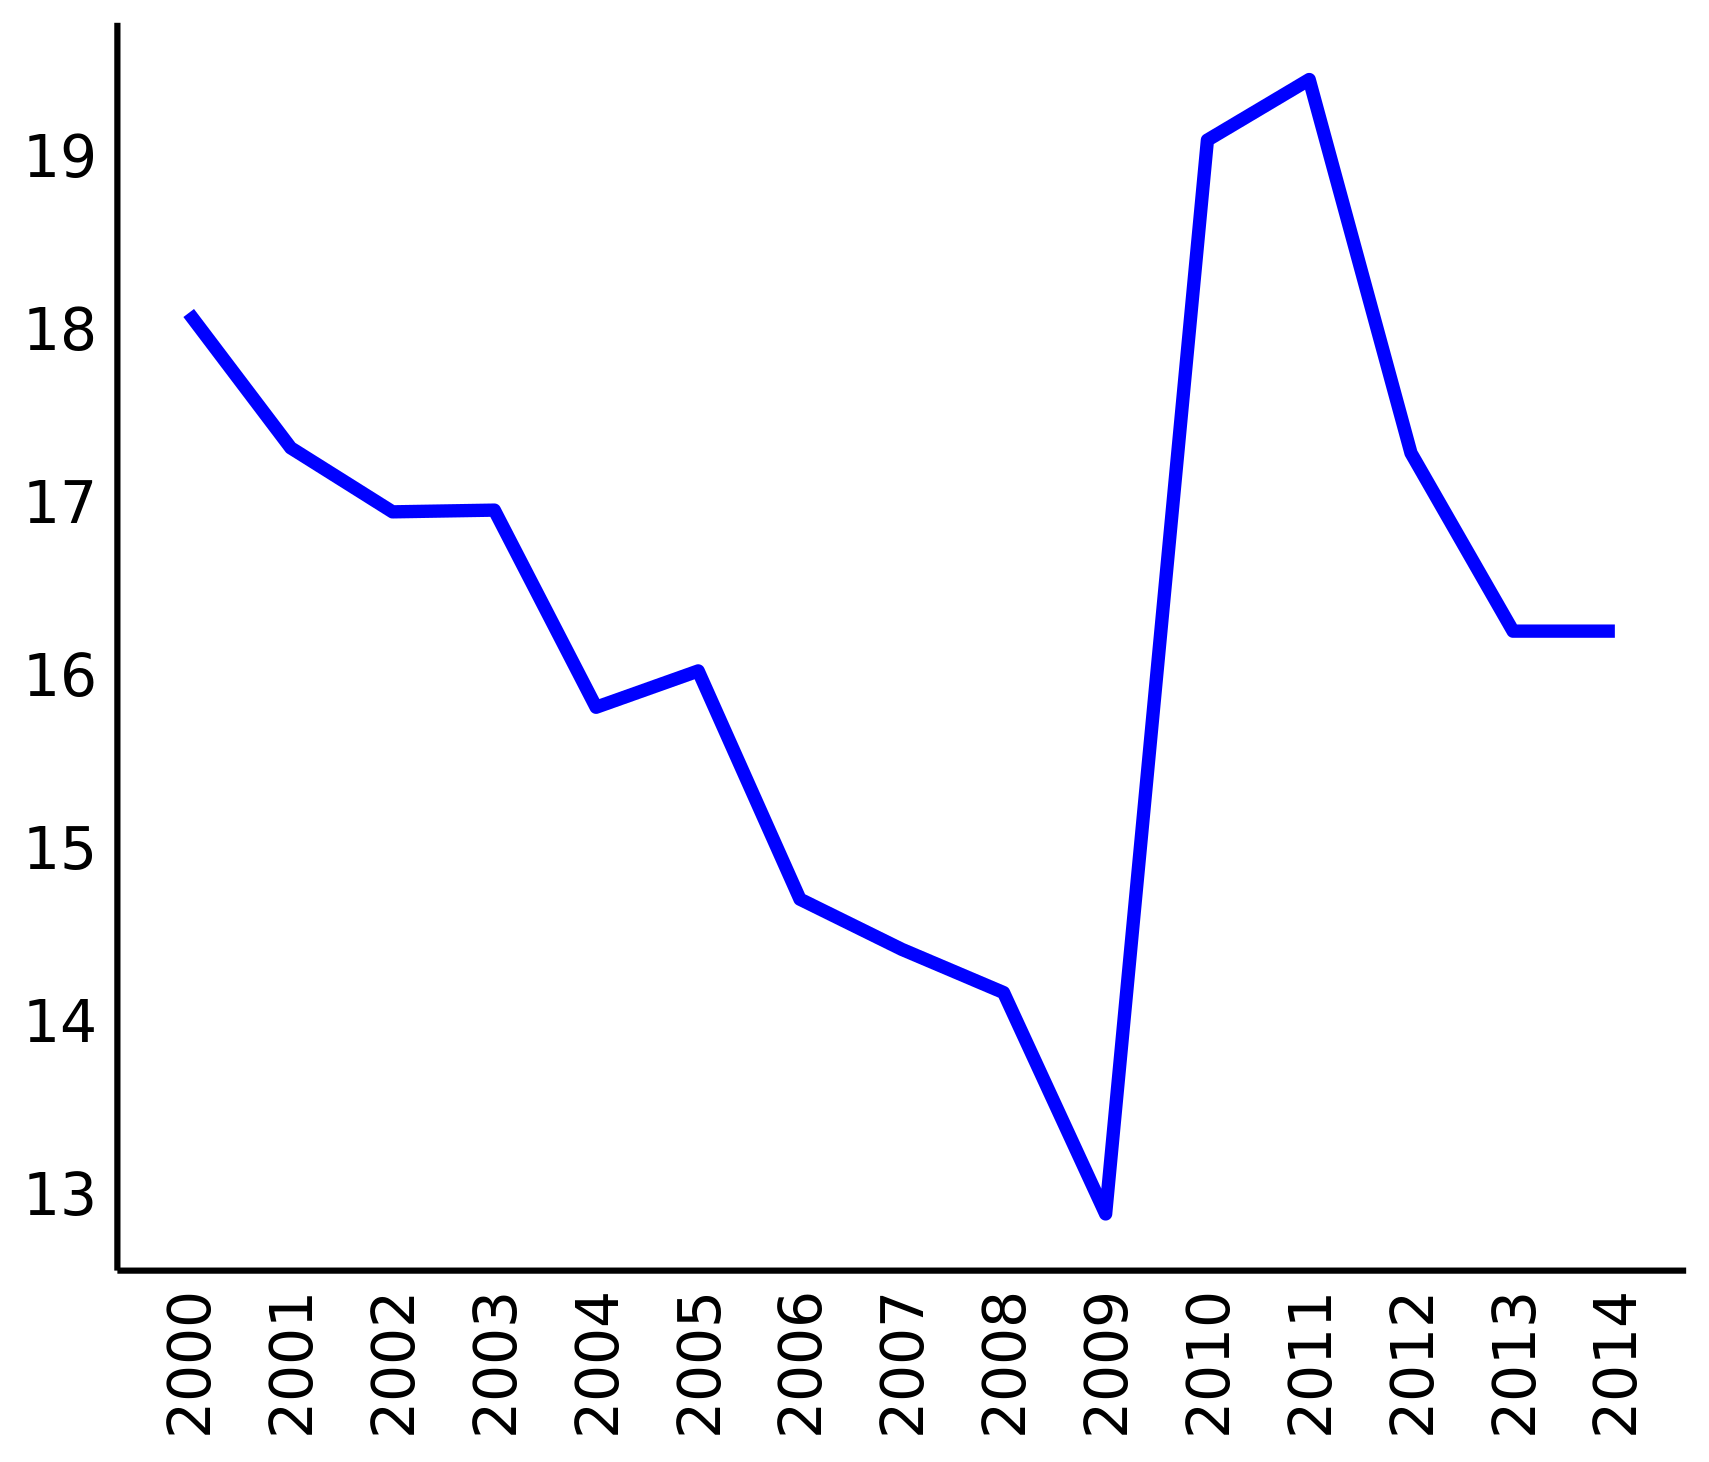
\includegraphics[height=1.8in]{2018-07-23_Plot_Part_10p40.png}\label{Razao}
%		} % Termina de incluir a figura fig2.pdf
%	\end{center}
%	\caption*{\textbf{Fonte:} Elaboração própria, dados do IPEADATA} 
%\end{figure} % Fecha o ambiente de figuras

\begin{figure}[htb]
\centering
\caption{Trajetória da razão entre a renda dos 10\% mais ricos e dos 40\% mais pobres em relação ao endividamento das famílias (2005-2014)}
\label{path}
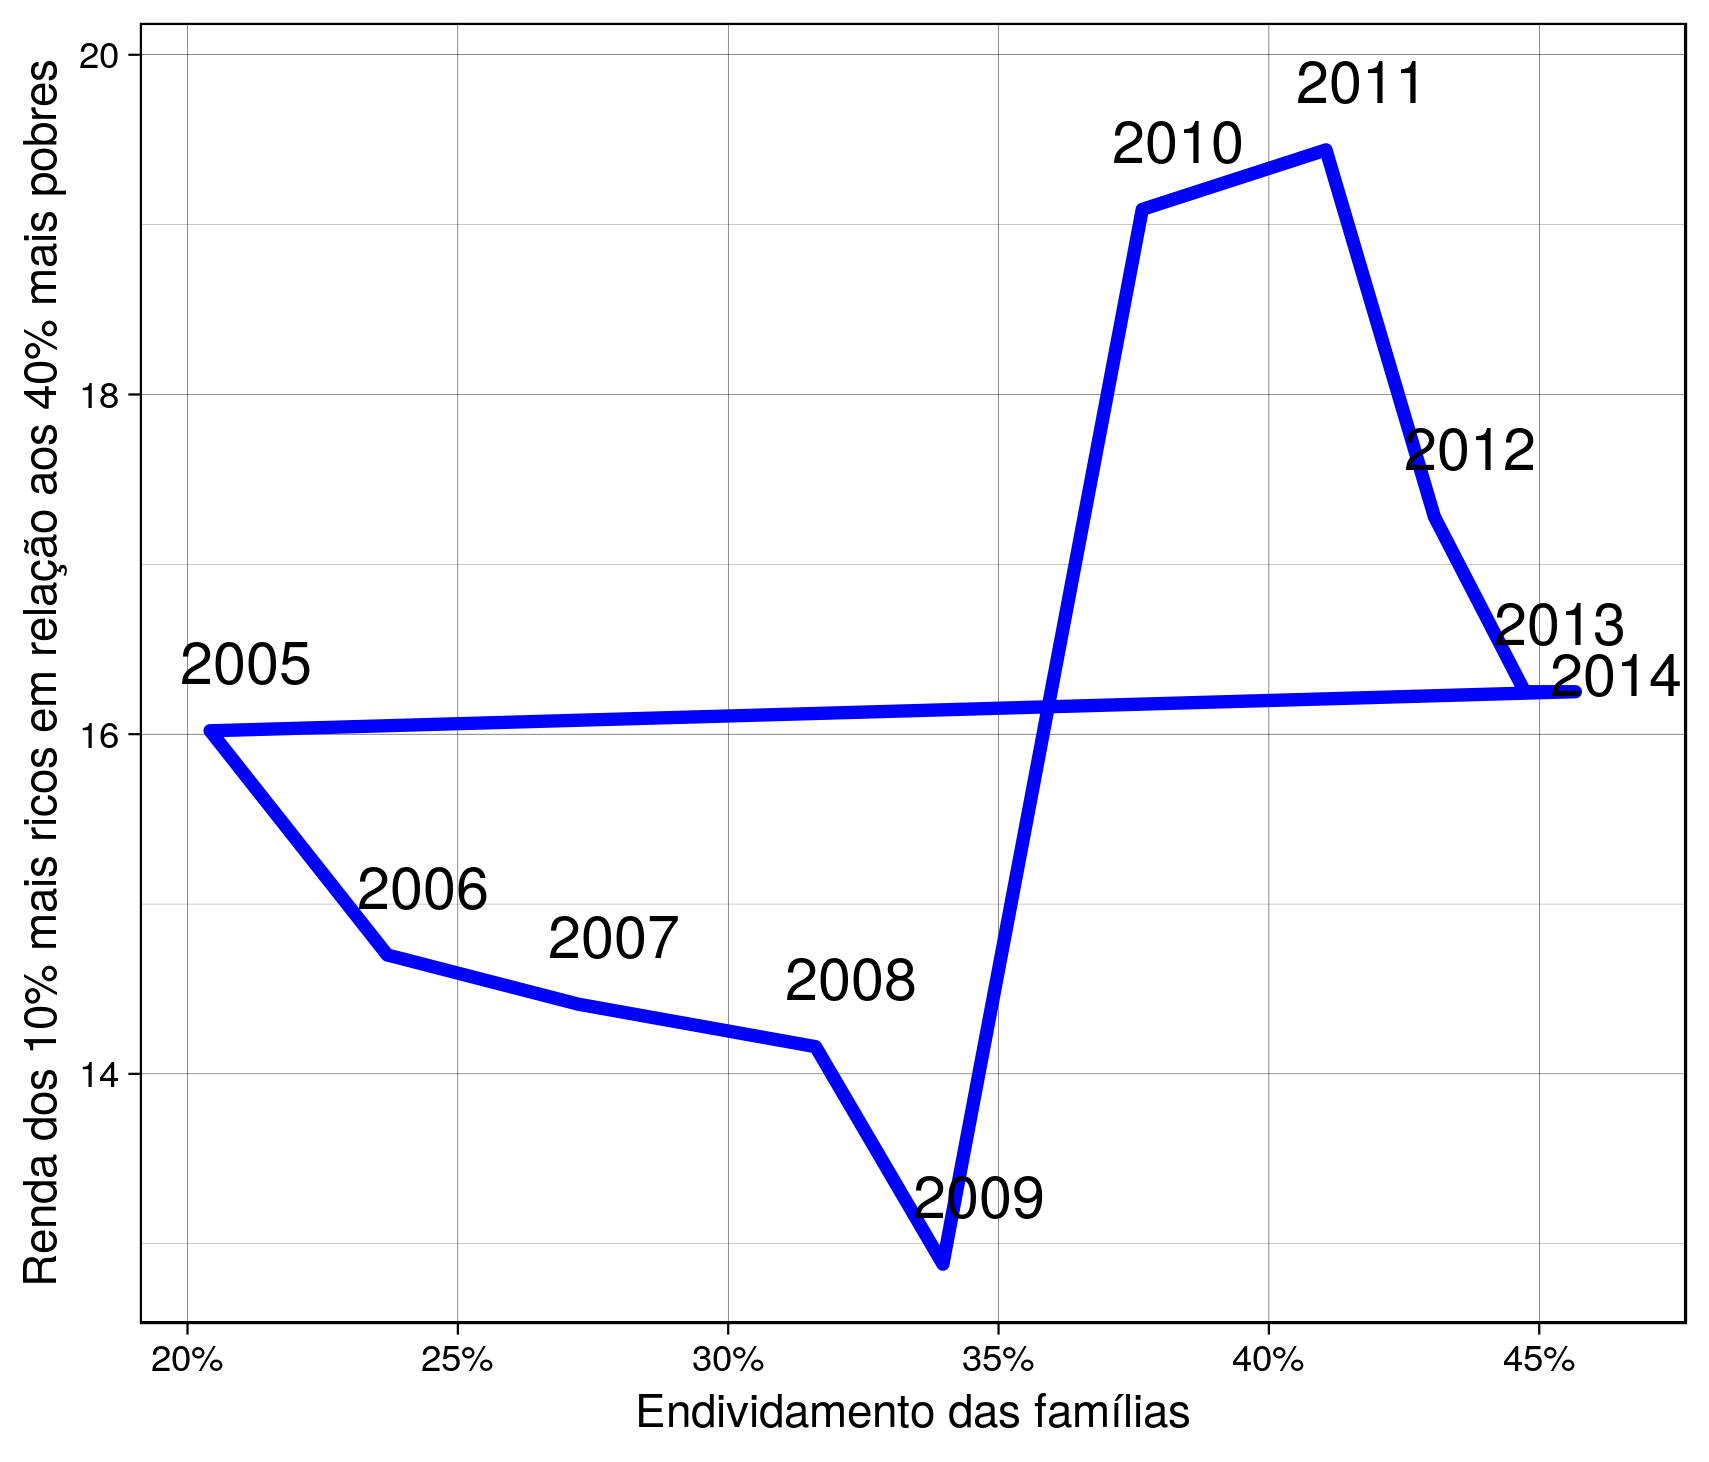
\includegraphics[width= .6\textwidth]{2018-07-23_Path_Endiv_10p40.png}\label{Razao}
\caption*{\textbf{Fonte:} IPEADATA e Bacen respectivamente}
\end{figure}

Isto posto e contrastando o caso americano, são evidenciadas mudanças redistributivas a favor dos estrados mais baixos de renda. No entanto, apesar de relevantes, essas mudanças podem não ser permanentes uma vez que não foram consolidadas as reformas estruturais necessárias \cite{carneiro_politica_2018}. Uma das manifestações da potencial efemeridade destas transformações é pontuada pelo acesso a um novo padrão de consumo por meio de maior acesso ao crédito e não via renda do trabalho\footnote{Isso não significa, no entanto, que não houveram ganhos salariais relevantes. Contraditoriamente, houve um aumento significativo dos salários que, por sua vez, aumentaram o colateral necessário, assim, permitindo acesso a canais de crédito.}.  

%=============================================================================
% 							JUSTIFICATIVAS
%=============================================================================


Diante disso, propõe-se investigar como a modernização do padrão de consumo das famílias acompanhada da presença crescente do crédito ao consumidor teve implicações relvantes sobre o crescimento econômico brasileiro.
Desta forma, a principal justificativa desta pesquisa é a importância dos efeitos e especificidades das mudanças relativas nas parcelas de renda no período recente (2000-2014). Em especial, destaca-se o aumento do endividamento privado junto  da democratização pelo consumo \cite{fontenelle_alcances_2016}. 

É digno de nota que, com a publicação da portaria MF N\textsuperscript{\underline{o}} 165/2016,
foram divulgados dados provenientes do Imposto sobre a Renda da Pessoa Física (IRPF) referentes aos anos de 2007 à 2013 que precisam ser melhor analisados. Tais informações trazem não apenas fontes adicionais para se estudar distribuição pessoal da renda como também uma base de comparação entre diferentes levantamentos domiciliares (\textit{i.e.} PNAD, Censo e POF).  
Portanto, outra justificativa desta pesquisa se dá pela relevância que tais estudos virão a ter no futuro.



\begin{comment}
%=====================================================
%				TEMPORARIAMENTE DESCARTADO
%=====================================================
\textcite{szymborska_household_2018}, por exemplo, afirma que pouco se sabe os tipos de riqueza responsáveis pela melhora (ou piora) da distribuição de renda das famílias. Partindo dos dados do \textit{Survey of Consumer Finances}, conclui que diferentes formas de riqueza afetam a distribuição de renda de maneira distinta.

Além disso, com a publicação da portaria
% TODO encontrar número da portaria
serão divulgados relatórios anuais (à partir de 2014) referentes aos dados provenientes do Imposto sobre a Renda da Pessoa Física (IRPF) que trarão não apenas fontes adicionais para se estudar distribuição pessoal da renda como também uma base de comparação entre diferentes levantamentos domiciliares (\textit{i.e.} PNAD, Censo e POF). Por mais que tais publicações fogem do recorte temporal deste projeto, foram divulgados dados referentes aos anos de 2007 à 2013 que precisam ser melhor analisados.
Portanto, outra justificativa desta pesquisa se dá pela relevância que tais estudos virão a ter no futuro em que esta investigação poderá trazer contribuições importantes. 


%Isso posto, o gráfico \ref{PIB} tenta ilustrar a dinâmica da economia brasileira em três movimentos: (A) internalização dos impactos decorrentes da crise internacional; (B) apequenamento do crescimento seguido do ajuste fiscal de 2015; e (C) comportamento da economia ao longo da crise. {\color{blue} Gráfico: Seria melhor plotar o endividamento das famílias realçando os mesmos pontos?}
%%No entanto, é importante destacar que não cabe aqui apresentar as razões nem a datação da crise recente, apenas elucidar sua trajetória.
%
%\begin{figure}[htb]
%	\begin{center}
%		\caption{Taxa de crescimento trimestral dessazonalizado (2001-2017) }
%		\label{PIB}
%		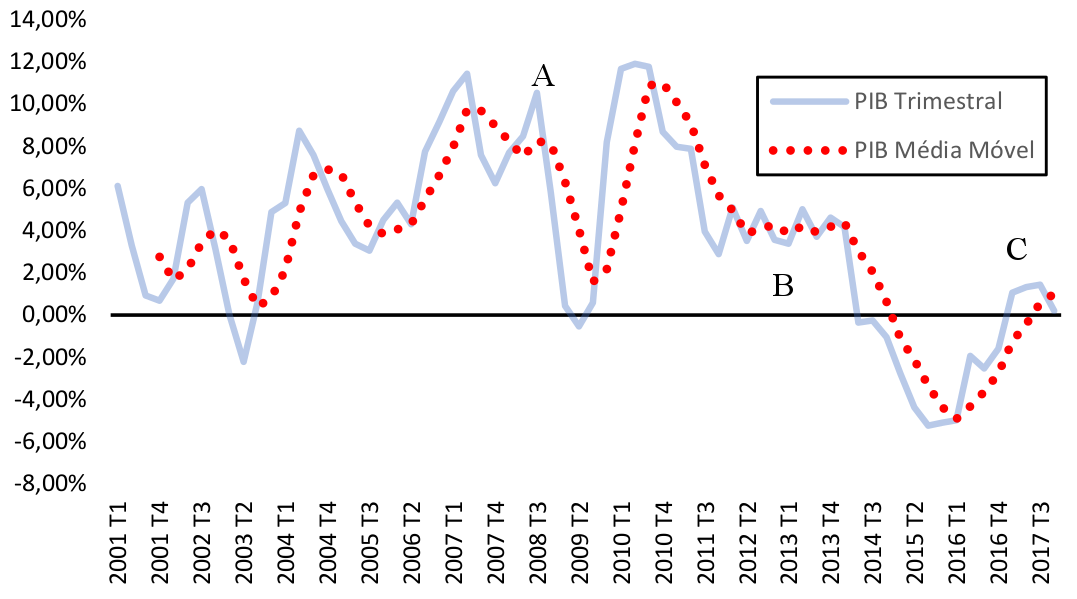
\includegraphics[width=.8\textwidth]{PIB_FAPESP}
%	\end{center}
%	\caption*{\textbf{Fonte:} Elaboração própria, dados do IPEADATA {\color{red} Rever fonte}}
%\end{figure}
%% TODO Verificar fonte
%
%Como esperado, essa crise está sendo alvo das mais diferentes 
%interpretações.
%Grosso modo, boa parte da literatura alveja as políticas econômicas como fonte desta desaceleração dinâmica, seja por serem elas austeras \cite{serrano_demanda_2015}, intervencionistas \cite{barbosa_filho_crise_2017}, estruturais \cite{bacha_saida_2017} ou até mesmo decorrentes das limitações da ossatura do Estado desenvolvimentista \cite{carneiro_economia_2017}. Com isso, indicam-se as fragilidades do padrão de crescimento brasileiro decorrentes das medidas inadequadas de política econômica, mas argumenta-se aqui que existem fatores estruturais que devem ser considerados.
%
%Esta pesquisa, portanto, tem um aspecto mais generalizante e tenta dar conta dos movimentos referentes às mudanças redistributivas tal como em \textcite{serrano_conflito_2018}. Vale notar que esta investigação não pretende dar uma explicação para o caso brasileiro recente, mas sim, contribuir para a compreensão deste episódio à luz da teoria monetária da distribuição de \textcite{pivetti_essay_1992}.


\end{comment}



